\section{Разработка библиотеки для синтаксического анализа графов}
\subsection{Библиотека Meerkat}
Meerkat --- это библиотека парсер-комбинаторов, разработанная на языке программирования Scala Али Афрузе и Анастасией Измайловой~\cite{IzmCombinator} для синтаксического анализа строк. Анализ осуществляется за $O(n^3)$, где $n$ --- длина последовательности, а также осуществляется построение компактного представления леса разбора Binarized Shared Packed Parse Forest (BSPPF). В ней решены проблемы левой рекурсии, а также экспоненциальной сложности за счет использования техники мемоизации и Continuation-Passing Style, предложенной Марком Джонсоном~\cite{MemoizationInTopDown}.

\subsection{Распознаватель в стиле парсер-комбинаторов}
В терминах данной библиотеки базовый распознаватель --- это функция типа $Recognizer$, которая определяется как функция $Int => Result[Int]$ (принимает значение типа $Int$ и возвращает значение типа $Result[Int]$). Базовый распознаватель --- это частичная функция, принимающая как аргумент позицию во входном потоке и возвращающее значение $success$, соответствующее успешному разбору и содержащее следующую позицию, или значение $failure$, соответствующее ошибке при анализе.

Для составления любой КС-грамматики необходимо реализовать набор базовых комбинаторов: анализаторы терминала и пустой строки, комбинаторы последовательности и правила. В библиотеке Meerkat для этих целей реализованы анализаторы $terminal$, и $epsilon$, а также комбинаторы $seq$ и $rule$ (см. листининг~\ref{parserAll}).

\begin{listing}
\caption{Распознаватели в стиле парсер-комбинаторов}
\label{parserAll}
\centering
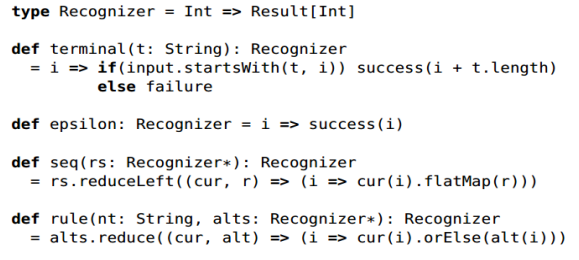
\includegraphics[width=0.9\textwidth]{Smolina/pics/combinators.png}
\end{listing}

Комбинатор $terminal$ возвращает распознаватель, который принимает индекс текущей строки и возвращает $success$ в случае, когда суффикс строки с текущего символа равен значению аргумента. Входной поток в данном случае предполагается глобальной переменной, но в реализации передаётся как параметр функции. 

Комбинатор $seq$ представляет собой последовательную композицию распознавателей. Он получает на вход текущую позицию и список распознавателей, затем применяет последовательно каждый из распознавателей к входному потоку, начиная с текущей позиции, и передает предыдущие результаты следующим распознавателям. Если какой-либо из распознавателей вернёт $failure$, то дальнейший разбор производиться не будет и комбинатор $seq$ вернёт $failure$. 

 Комбинатор $rule$ используется, чтобы определить нетерминал с именем $nt$ и списком распознавателей $alts$, которые представляют из себя альтернативы правила грамматики. Данный комбинатор принимает как параметр текущую позицию во входном потоке и применяет каждый анализатор к этому символу, пока хотя бы один не вернёт $success$. 

Для того чтобы в строго типизированных языках можно было реализовать рекурсивные распознаватели, введен дополнительный комбинатор $fix$ (см. листинг~\ref{fix}) --- комбинатор неподвижной точки.

\begin{listing}
\caption{Комбинатор fix}
\label{fix}
\centering
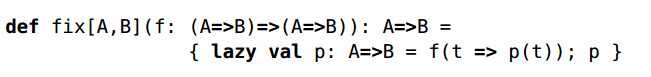
\includegraphics[width=0.9\textwidth]{Smolina/pics/fix.png}
\end{listing} 

Комбинирование элементарных анализаторов и представленных выше парсер-комбинаторов позволяет анализировать произвольную КС-грамматику и избежать зацикливания обработке леворекурсивных правил~\cite{GLL}.

\subsection{Полный перебор с использованием Continuation-Passing Style}
У базовых распознавателей есть недостатки: более высокий приоритет у первого распознавателя альтернативы и детерминизм. Из-за более высокого приоритета первого распознавателя анализ строки ``ab'' относительно грамматики $S \rightarrow A \ \$; A \rightarrow a \mid a \ b$ завершится ошибкой --- $failure$: первая альтернатива нетерминала $A$ распознает односимвольный префикс строки, после чего произойдет ошибка при проверки на конец строки, и второй распознаватель не будет применен к началу строки. Детерминизм означает, что результатом успешного распознавания всегда является единственное решение, в то время как их может быть и несколько. Порождение всех возможных выводов строки возможно при помощи техники Continuation-Passing Style (CPS).

При программирования в стиле Continuation-Passing передача управления происходит через механизм продолжений. Продолжение в данном контексте представляет собой функцию высшего порядка, содержащую информацию о состоянии программы в конкретный момент времени, которое возможно сохранить и вызвать позже для перехода в данное состояние.

Для преобразования базовые распознаватели в CPS авторы библиотеки Meerkat изменили тип $Result[T]$ и сопровождающие его функции $success$ и $failure$. Любой результат теперь должно быть возможным представить как композицию двух функций, используя метод $flatMap$, или как комбинацию двух возможных альтернатив, используя метод $orElse$. Реализация в библиотеке Meerkat представлена в листинге~\ref{result}.

\begin{listing}
\caption{Result[T] для CPS распознавателей}
\label{result}
\centering
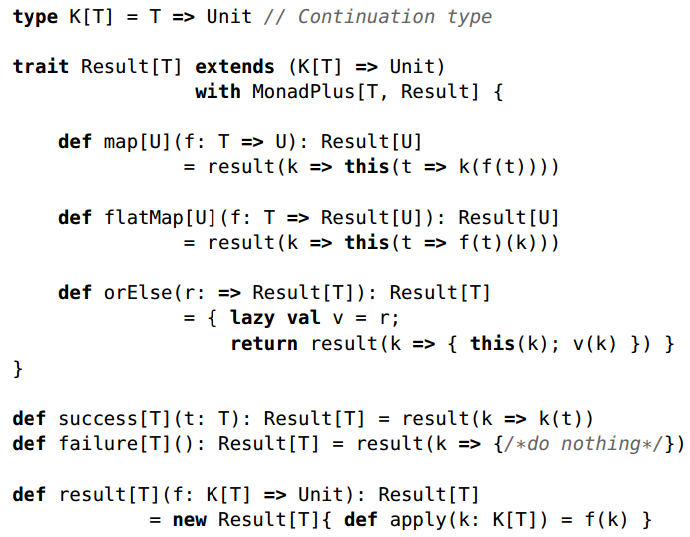
\includegraphics[width=0.8\textwidth]{Smolina/pics/result.png}
\end{listing}

CPS распознаватель принимает на вход позицию и возвращает функцию типа $Result[T]$. Данная функция принимает на вход продолжение типа $K[Int]$ и возвращает $Unit$. Продолжение в данном случае является функцией-остатком процесса распознавания. Вместо возвращения значения, распознаватель возвращает либо $success$, вызывая продолжение со следующей позиции, либо $failure$, не вызывая продолжения. Такая реализация осуществляет перебор всех возможных решений. 

\subsection{Мемоизация и поддержка левой рекурсии}
Наивный перебор всех возможных решений приводит к экспоненциальной сложности алгоритма. Библиотека Meerkat использует мемоизацию для обеспечения полиномиальной сложности, а также для решения проблемы с леворекурсивными нетерминалами.

 Мемоизацией называют механизм, который позволяет сохранять вычисленные результаты и в дальнейшем переиспользовать их. При применении распознавателя, алгоритм в первую очередь проверяет в таблице мемоизации, не было ли вычислено значение данного распознавателя в данной позиции ранее. Если вычисление происходит в первый раз, результат записывается в таблицу мемоизации. Иначе распознаватель не выполняется, а результат его работы берется из таблицы. В листинге~\ref{memo} представлен такой механизм для техники CPS, реализованный в библиотеке Meerkat.

 Функция $memo$ превращает произвольный распознаватель CPS в мемоизированный CPS-распознаватель. Мемоизированный CPS-распознаватель при каждом вызове в позиции i обращается к таблице $table$. Таблица $table$ содержит функцию для работы с продолжениями для каждого символа. В случае, когда для позиции i применяется немемоизированый распознаватель в первый раз, его модификация сохраняется и представляет собой переменную res. Результат распознавателя вычисляется только после обновления таблицы $table$. Если распознаватель был вызван в данной позиции раньше, его результат возвращается из $table$. Таким образом решается проблема экспоненциального взрыва.

\begin{listing}
\caption{Мемоизация для CPS}
\label{memo}
\centering
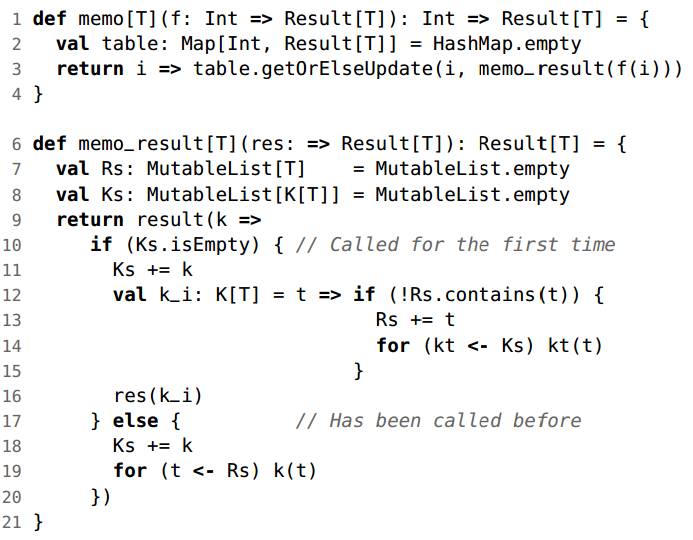
\includegraphics[width=0.8\textwidth]{Smolina/pics/memo.png}
\end{listing}

%%%%%%%%%%%%%%%%%%%%%%%%%%%%%%%%%%%%%%%%%%%%%%%%%%%%%%%%%%%%%%%%

Каждый CPS-распознаватель оперирует двумя списками: $Rs$ и $Ks$. Список $Rs$ содержит все позиции входа, созданные немемоизированным распознавателем, когда он достигает успеха, будучи примененным к позиции $i$. Список $Ks$ содержит все продолжения, которые передаются в функцию $memo\_result$, когда они вызываются в позиции $i$. Если мемоизированный распознаватель вызывается в первый раз, текущее продолжение добавляется к $Ks$, а исходный немемоизованный распознаватель вызывается с новым продолжением $k\_i$. Продолжение $k\_i$ создается только после первого вызова мемоизированного распознавателя в $i$. Каждый раз, когда немемоизированный распознаватель завершается с успехом в позиции $i$, $k\_i$ проверяет, была ли эта входная позиция получена как результат раньше, если нет, сначала записывает ее в $Rs$, а затем запускает все записанные продолжения. С другой стороны, если вызванный мемоизированный результат был вызван ранее, текущее продолжение $k$ добавляется к $Ks$ и вызывается для каждой входной позиции,записанной в $Rs$.

Теперь, когда мемоизированный леворекурсивный CPS-распознаватель вызывается во входной позиции $i$, его завершение гарантируется, поскольку соответствующий немемоизированный распознаватель никогда не будет вызван в $i$ более одного раза. В то же время, часть пути выполнения, которая привела к леворекурсивному вызову и может создавать новые позиции для левого рекурсивного распознавателя в $i$, эффективно записывается как продолжение. Каждое продолжение фиксирует следующий шаг в альтернативе после завершения текущего вызова. Продолжения будут выполняться для любой входной позиции, создаваемой леворекурсивным распознавателем в позиции $i$, до тех пор, пока создаются новые позиции ввода~\cite{IzmCombinator}. Таким образом решается проблема левой рекурсии.

\subsection{ Библиотека для синтаксического анализа графов}
Основной задачей работы является разработка решения для синтаксического анализа графа, которое позволяет не только писать запросы непосредственно в коде программы, но и получать результат этих запросов в компактной форме SPPF.

Данная работа требует решения промежуточных шагов.
\begin{enumerate}
\item Входным типом данных библиотеки Meerkat являются строки, необходимо изменить его на граф.
\item Строки можно рассматривать как линейную последовательность ребер и вершин, поэтому далее необходимо преобразовать библиотеку для анализа последовательности вершин с несколькими исходящими ребрами (деревья) с различными метками, а также графа с циклами.
\item Необходимо преобразовать библиотеку для анализа графов с одинаковыми ребрами, исходящими из одной вершины.
\item Необходимо добавить функциональность для решения частных задач синтаксического анализа.
\item Необходимо добавить функциональность для работы с графовой базой данных Neo4j.
\end{enumerate}

\subsubsection{Изменение входного типа данных на граф}


Входной последовательностью в библиотеке Meerkat являются строки. Для работы с ними разработчиками библиотеки был разработан класс $Input$, который в конструкторе получает строку. Для добавления нового типа входных данных класс $Input$ был преобразован в интерфейс $Input$, который имеет следующие методы:
\begin{itemize}
\item $startWith$: принимает на вход строку $prefix$ и позицию в последовательности $n$. Проверяет, является ли prefix префиксом суффикса строки, начинающегося с позиции $n$;
\item $matchRegex$: принимает на вход регулярное выражение и позицию в последовательности. Проверяет, содержится ли в суффиксе строки с позиции $n$ строка, удовлетворяющая данному регулярному выражению.
\end{itemize}

Класс $InputString$ реализует интерфейс для строки, класс $InputGraph$ --- для графа. Для графа был разработан интерфейс $IGraph$, задающий методы необходимые для реализации класса $InputGraph$. Для тестирования данный интерфейс был реализован для типа данных $scalax.collection.Graph$~\cite{Graph}. Это простая в использовании реализация графа, в которой кратко и наглядно можно представить узлы и связи между ними.

\subsubsection{Преобразование системы для анализа дерева и графа с циклами}


Дерево представляет собой связный граф, в котором нет циклов. Пример дерева представлен на рис.~\ref{Graph1}. На данном этапе метки на ребрах, исходящих из одной вершины, должны быть различны. Необходимо преобразовать библиотеку для осуществления синтаксического анализа деревьев.

\begin{figure}

 \centering
 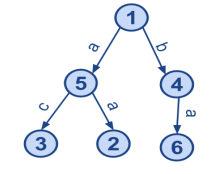
\includegraphics[width=0.4\textwidth]{Smolina/pics/Graph1.png}
 \caption{Дерево $A_1$}
 \label{Graph1}
\end{figure}

Для решения данной задачи необходимо преобразовать синтаксический анализатор терминала (см. листинг~\ref{parser1}). Данный метод принимает на вход строку-шаблон (длины $k$) и позицию во входной последовательности ($n$). Если существует подстрока, начинающаяся с позиции $k$ и совпадающая с шаблоном, то возвращается значение $success$, содержащее позицию, с которой следует продолжить разбор --- $k+n$. При обработке узла дерева просматриваются все исходящие ребра и проверяется соответствие их меток со значением терминала. Если существует ребро с соответствующим терминалом, необходимо вернуть вершину, в которую направлено ребро. Так как не для всех исходящих ребер анализ успешен, а для ситуаций успешного анализа надо возвращать позицию, то тип данных метода $startWith$ необходимо изменить с $Boolean$ на $Option[Int]$.

В графах с циклами, в отличие от деревьев, в одну и ту же вершину может существовать несколько путей, которые могут иметь циклическую структуру. В наивной реализации парсер-комбинаторов каждый путь приходилось бы пересчитывать заново, а в случае с циклом вычисление бы никогда не завершилось. Однако применение техники мемоизации совместно с CPS гарантирует вычисление каждого анализатора в каждой вершине не более одного раза. Для каждой вершины существует свой набор продолжений, который комбинируется и переиспользуется. Благодаря этим свойствам дальнейших изменений для поддержания графов с циклами не потребовалось. Циклы в графе обрабатываются подобно леворекурсивной грамматике.

Таким образом решена задача синтаксического анализа для деревьев и графов с циклами. Проиллюстрируем полученные результаты на примере 1.

\textsc{Пример 1.} 
Входной граф представлен на рис.~\ref{Graph2}, данный граф цикличен. Стартовой вершиной считаем вершину 0. Результат синтаксического анализа в соответствии с грамматикой $G_1$ представлен на рисунке~\ref{grmG4}.

\begin{figure}
 \centering
 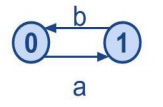
\includegraphics[width=0.2\textwidth]{Smolina/pics/Graph2.png}
 \caption{Циклический граф $A_2$}
 \label{Graph2}
\end{figure}

\begin{listing}
\caption{Грамматика $G_1$}
\label{grmG4}
\centering
$\begin{array}{rl}
E \rightarrow a \ b \ E \ | \ a \ b
\end{array}$
 \end{listing}

\begin{figure}
 \centering
 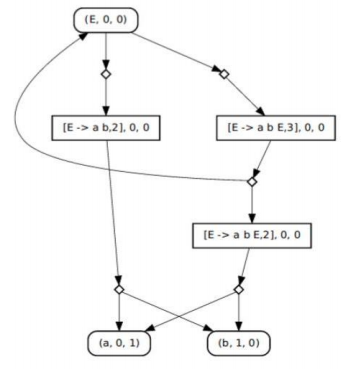
\includegraphics[width=0.4\textwidth]{Smolina/pics/Tree1.png}
 \caption{Результат применения анализатора $E$ к графу $A_2$}
 \label{Tree1}
\end{figure}

Результатом синтаксического анализа преобразованной библиотекой Meerkat является синтаксический лес разбора, представленный на рисунке~\ref{Tree1}. Из корневой вершины исходит две ветви, два возможных решения. Первое решение строка ``ab''. Второе решение соответствует рекурсивному правилу грамматики с префиксом ``ab'' с левой ветвью указывающей на корень дерева, представляя собой бесконечное множество возможных деревьев разбора.

\subsubsection{Преобразование системы для анализа графов с одинаковыми ребрами из одной вершины}


Ранее требовалась уникальность исходящих ребер из одной вершины. В этом случае из каждой вершины может существовать единственный путь, начинающийся с данного терминала. Если отказаться от данного ограничения, то таких путей может существовать несколько или не существовать вовсе, поэтому необходимо изменить тип и реализацию метода $startWith$. Теперь результатом его работы будет тип $Set[Int]$. Когда множество оказывается не пусто, будем считать, что разбор прошел успешно ($success$) иначе --- завершился ошибкой ($failure$).

Метод $terminal$ также требует изменений. Все успешные пути, полученные методом $startWith$, комбинируются при помощи $orElse$ класса
$Result$. В результате чего получаем единственное продолжение, которое возвращается для дальнейшей обработки. Пример 2 демонстрирует работу новой реализации.

\textsc{Пример 2.} 
Входной граф $A_3$ представлен на рисунке~\ref{Graph3}. Из стартовой вершины 0 исходят 3 ребра с одинаковыми метками. Проведем синтаксический анализ в соответствии с грамматикой $G_2$ в листинге~\ref{grmG5}.

\begin{figure}
 \centering
 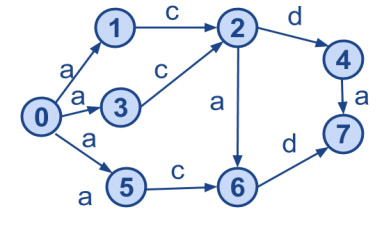
\includegraphics[width=0.6\textwidth]{Smolina/pics/Graph3.png}
 \caption{Граф $A_3$}
 \label{Graph3}
\end{figure}

\begin{listing}
\caption{Грамматика $G_2$}
\label{grmG5}
\centering
$\begin{array}{rl}
E \rightarrow a \ c \ d \ E \ | \ a \ d
\end{array}$
 \end{listing}

\begin{figure}
 \centering
 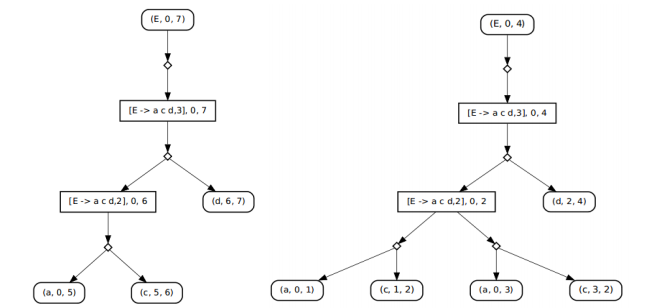
\includegraphics[width=\textwidth]{Smolina/pics/Trees2.png}
 \caption{Результат применения анализатора $E$ к графу $A_3$}
 \label{Trees2}
\end{figure}

Результат работы представлен на рис.~\ref{Trees2}. В графе $A_3$ из вершины 0 существуют 3 пути, соответствующие грамматике $G_2$ (0-5-6-7, 0-1-2-4 и 0-3-2-4). В результате получен граф SPPF, где несколько вершин выделены как начальные. Вершины, соответствующие общим подпутям при этом переиспользуются.

SPPF представляет собой компактное представление множества деревьев разбора одной строки. В случае синтаксического анализа графов необходимо построить множество деревьев разбора множества строк, что возможно сделать, если модифицировать SPPF таким образом, чтобы у него было несколько ``корневых'' узлов. За счет такого определения можно обеспечить переиспользование деревьев разбора для общих подпутей.

В библиотеке Meerkat во время анализа строится структура данных $SPPFLookup$. Она представляет собой множество уникальных узлов, создаваемых во время анализа, которые ссылаются друг на друга. При успешном результате один или несколько узлов, как в нашем случае, берутся как корни дерева.

\subsubsection{Функциональность для решения частных задач синтаксического анализа}

Ранее мы обсуждали поиск всех путей в графе, удовлетворяющих заданным ограничениям. Существуют и другие семантики запросов, при которых необходимо идентифицировать некое подмножество всех путей, удовлетворяющих ограничениям. Такими семантиками являются~\cite{Hellings}:

\begin{itemize}
\item поиск всех путей в графе;
\item поиск путей, начинающихся с какой-либо вершины из данного
множества;
\item поиск путей, завершающихся в какой-нибудь вершине из данного
множества;
\item поиск путей, начинающихся в какой-нибудь вершине множества
начальных вершин и заканчивающихся в вершине из множества
конечных вершин.
\end{itemize}

Для нахождения решений, удовлетворяющих каждой из данных семантик, не требуется изменений в процессе разбора. После построения $SPPFLookup$ необходимо произвести фильтрацию стартовых нетерминальных символов в соответствии с семантикой запроса, то есть выбрать корневые вершины, которые удовлетворяют требованиям. В итоге все вычисления производятся один раз и уже из полученных результатов выбираются необходимые. 

\subsubsection{Интеграция библиотеки с графовой базой данных Neo4j}

Было решено применить результат работы библиотеки для синтаксического анализа графов к существующей графовой базе
данных. Нами была выбрана графовая база данных Neo4j~\cite{Neo4j}. Она обладает наглядным и удобным в использовании интерфейсом, имеет REST API для доступа из любого языка программирования и большое количество пользователей по всему миру.

Для интегрирования реализован класс $Neo4jGraph$, реализующий методы интерфейса $IGraph$. Класс использует REST API для работы с базой данных, предоставленное компанией Neo4j. В качестве индексов во входном потоке используется уникальный идентификатор вершин графа.

\textsc{Пример 2.} 
Для тестирования была взята графовая база данных Wine. Фрагмент представлен на рис.~\ref{GraphWine}. Каждая вершина представляет собой вид вина, регион или тело вина. Между ними представлены два вида связи: 
\begin{itemize}
\item $locatedIn$ указывает на расположение объекта, из которого исходит ребро;
\item $hasBody$ указывает на цвет вина
\end{itemize}

\begin{figure}
 \centering
 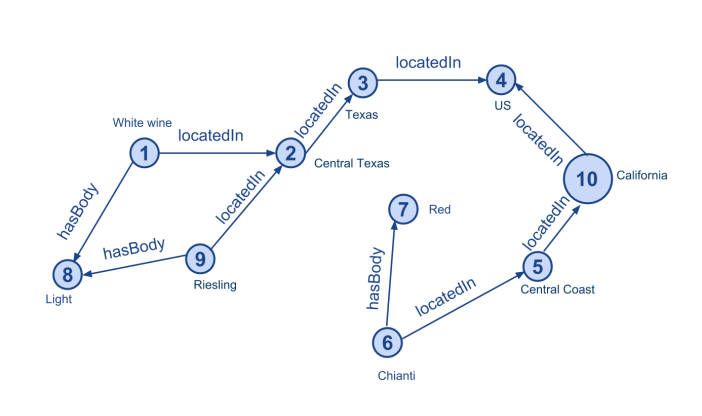
\includegraphics[width=0.9\textwidth]{Smolina/pics/GraphWine.png}
 \caption{Фрагмент графовой базы данных Wine}
 \label{GraphWine}
\end{figure}

Для того, чтобы узнать в каких регионах производят Riesling, необходимо выполнить запрос представленный в листинге~\ref{grmG6}. 

\begin{listing}
\caption{Запрос: определение региона}
\label{grmG6}
\centering
$\begin{array}{rl}
S \rightarrow locatedId \ S | \ locatedIn
\end{array}$
 \end{listing}

В процессе работы было получено 3 пути, начинающиеся с вершины $9$ и заканчивающиеся в вершинах $2, 3, 4$. Соответствующие этим вершинам названия, соответствуют расположению регионов, где производится вино Riesling: Central Texas, Texas, US.
 
 \textsc{Пример 3.}

Другой пример, демонстрирующий необходимость в запросах, представленных в КС-грамматиках --- это поиск потомков одного поколения.

База данных моделирует семейное древо (см. рис.~\ref{GraphFamily}). Требуется найти всех потомков одного поколения: например, всех братьев и сестер конкретного узла. Нахождение всех этих потомков может быть произведено запросом в виде грамматики (см. листинг~\ref{grmG7}). Данная грамматика представляет собой язык правильных скобочных последовательностей, где одна скобка --- отношение ``ребенок'', другой --- отношение ``родитель''. Технически, данные в базе данных представлены таким образом, что существуют только переходы от предков к потомкам, поэтому отношение ``ребенок'' необходимо симулировать как обратное ребро. Для обработки данной ситуации был добавлен комбинатор ``not'', который осуществляет анализ в обратном направлении: от узла, в которое входит ребро, в узел, из которого исходит ребро.

\begin{figure}
 \centering
 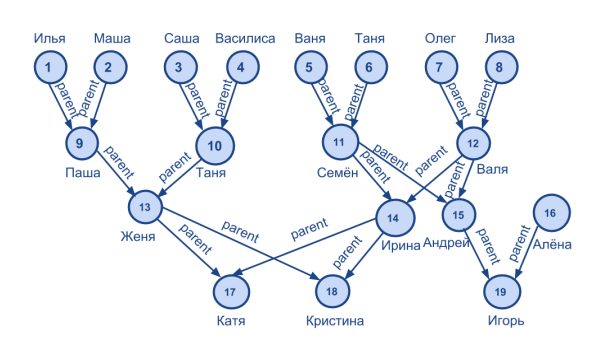
\includegraphics[width=0.8\textwidth]{Smolina/pics/GraphFamily.png}
 \caption{Фрагмент графовой базы данных ``Семейное древо''}
 \label{GraphFamily}
\end{figure}

\begin{listing}
\caption{Запрос: определение потомков одного поколения}
\label{grmG7}
\centering
$\begin{array}{rl}
S \rightarrow child \ S \ parent| \ epsilon
\end{array}$
 \end{listing}

Найдем всех потомков одного поколения для Кати из базы данных ``Семейное древо''. Для этого запишем запрос в виде грамматики
представленной в листинге~\ref{grmG8}.

\begin{listing}
\caption{Запрос: определение потомков одного поколения}
\label{grmG8}
\centering
$\begin{array}{rl}
S \rightarrow - \ parent \ S \ parent| \ epsilon
\end{array}$
 \end{listing}

В результате работы синтаксического анализатора было получено три дерева: дерево из вершины $17$ в вершину $17$, из $17$ в $18$ и из $17$ в $19$. Это говорит о том, что в одном поколении находятся Катя, Кристина и Игорь. Также из полученных деревьев можно узнать, кто является ближайшим общим родственником.
